\chapter{Problématiques émergentes et choix technologiques}

\section{Introduction}

Dans ce mémoire, nous avons décrit divers modèles et principes de conception
d'un système sensible au contexte et présenté une multitude d'intergiciels et
d'approches distribuées pour simplifier la configuration d'applications
sensibles au contexte. De cet état de l'art se dégagent plusieurs problématiques
dans le développement d'un système de configuration basé sur le contexte
auxquelles nous tenterons d'apporter une solution.

\section{Besoin d'un nouvel intergiciel}

Le besoin d'un nouvel intergiciel se fait ressentir du coté de l'implémentation.
Les technologies intergicielles actuelles ne sont pas adaptées pour le prise en
considération des restrictions imposées pas la mobilité et les systèmes
environnementaux intelligents : connexions volatiles, traitements et restrictions
mémoire sur les périphériques mobiles, canaux de communication étroits, écrans
réduits, mécanismes d'entrées restreintes, et la liste continue. Il existe
néanmoins une gamme d'implémentations de systèmes sensible au contexte dans la
littérature avec quelques prototypes fonctionnels :

\begin{itemize}
    \item \textbf{Hydrogen} \cite{hofer_context-awareness_2003}: 
        une architecture en trois couches.
    \item \textbf{Gaia} \cite{chetan_mobile_2005}: 
        une autre infrastructure intergicielle, étends les caractéristiques
        génériques des systèmes d'exploitation pour y incorporer la
        sensibilité au contexte.
    \item \textbf{CybreMinder} \cite{abowd_context-aware_2002}: 
        un système sensible au contexte permettant de générer des messages
        de rappel.
    \item \textbf{Context Toolkit} \cite{dey_conceptual_2001}: 
	    une architecture basée sur les widgets.
\end{itemize}

\subsection{Elaboration d'un framework de gestion de configuration}

La gestion de la configuration est le processus de contraindre le comportement
d'un réseau de machines de manière à ce que le comportement de chaque machine
soit conforme aux politiques et lignes directrices prédéfinies, et
accomplisse les objectifs d'entreprise prédéterminés. Cela implique :

\begin{itemize}
  \item Des personnes
  \item Un outil gestion de configuration ``zéro`` (exemple: CfEngine)
  \item Un ensemble ce machines interconnectées
  \item Un ensemble de processus de configuration destiné à aboutir à un système
	  conforme à la politique en vigueur.
\end{itemize}

Les paramètres de configuration peuvent être la permission d'un fichier,
l'adresse d'un carte réseau, le type de système de fichier pouvant être monté
sur un volume disque.

La possibilité d'automatiser par exemple la configuration des réseaux IP
(Internet Protocol) en utilisant une technologie sémantique est très
prometteuse. L'initiative connexe de créer un environnement de réseau de
capteurs basé sur le ontologies semble également être une solution viable.
La plupart des organisations aujourd'hui n'ont aucun procédé systématique pour
gérer leurs informations de configuration. Cela signifie que des informations
comme l'adresse IP d'une machine et le statut de son service réseau sont
stockées de manière dispersée et désorganisée. Certains outils de supervision
tels que Nagios présentent une manière de réorganiser ces informations provenant
de sources dispersées. 

\subsection{Utilisation d'une base de gestion de configuration}

L'idée d'utiliser une CMDB (Configuration Management Database) est également une
alternative permettant de solutionner le problème ci-dessus. La base de données
de gestion de configuration est une base unifiant les composants d'un système
informatique. Elle permet de comprendre l'organisation entre ceux-ci et de
modifier leur configuration. La CMDB est un composant fondamental d'une
architecture basé sur les application doté d'un gestionnaire de configuration
centralisé. 

Cette nouvelle façon de renforcer l'efficacité de la gestion des connaissances
dans le domaine de la gestion de configuration, nécessite la possibilité
d'extraction automatique de données à partir d'emplacements de stockage
précédents et la possibilité de mise à jour automatique de stockages permanents
tels que la CMDB afin d'augmenter la qualité de l'information sous-jacente.

Ces deux fonctionnalités, à savoir, l'extraction automatique des
données et également la mise à jour automatique des informations stockées
doivent impérativement être implémentées. Mais le besoin pour un gestionnaire
d'informations de plus haut niveau est tout de même mentionné dans de nombreuses
littératures.

\subsection{Conception d'une ontologie de gestion de configuration}

La structure de l'information de configuration stockée dans une CMDB et dans
d'autres fichiers sera représentée en concordance avec les standard de OWL.
Cette structure de domaine de connaissance sera implémentée comme une promesse
de structure d'information. La structure d'information initiale s'inspirera très
largement des dictionnaires fournis par le gestionnaire de configuration EOLE
Créole. Créole est un composant majeur des distributions EOLE permettant
l'agrégation et la mise en corrélation des données de configuration de chacun
des modules. Un présentation plus détaillée de cette technologie est donnée en
annexe \ref{appendix:EOLE}.

\section{Représentation des informations de contexte}

L'une des principales innovations à apporter dans les infrastructures
d'applications sensibles au contexte réside dans l'introduction d'une interface
présentant un niveau d'abstraction élevé. Cela permettrait de représenter la
connectivité des composants applicatifs avec les politiques de haut niveau qui
la régissent. Cette couche doit rester simple d'utilisation pour les
développeurs d'applications, et le modèle améliorer simultanément
l'automatisation et la sécurité.

\subsection{Conception d'un ontologie de contexte}
\label{sec:ontology}

La représentation des informations de contexte est grande préoccupation. Nous
avons présenté dans ce mémoire une approche basée sur les ontologie très
générique. Elle est basée sur quatre concepts fondamentaux : utilisateur,
environnement, plateforme et ressources. Actuellement, les ontologies sont
surtout utilisées pour permettre la communication entre les différents
périphériques dans le même réseau. Comme proposé par le ContextUML
\cite{sheng_contextuml:_2005}, le Langage de Modélisation Unifié (UML) peut
également être utilisé pour modéliser le contexte. Ces modèles pourraient être
utilisés pour séparer la définition et l'information liée au contexte de
l'implémentation spécifique. Il existe d'autres caractéristiques qui font que
l'information de contexte est difficile à modéliser : comme abordé précédemment,
il est parfois nécessaire de différencier une information statique d'une
information dynamique. 

\subsubsection{Entités principales de l'ontologie}

%\begin{wrapfigure}{r}{.7\textwidth}
\begin{figure}[h]
    \centering
    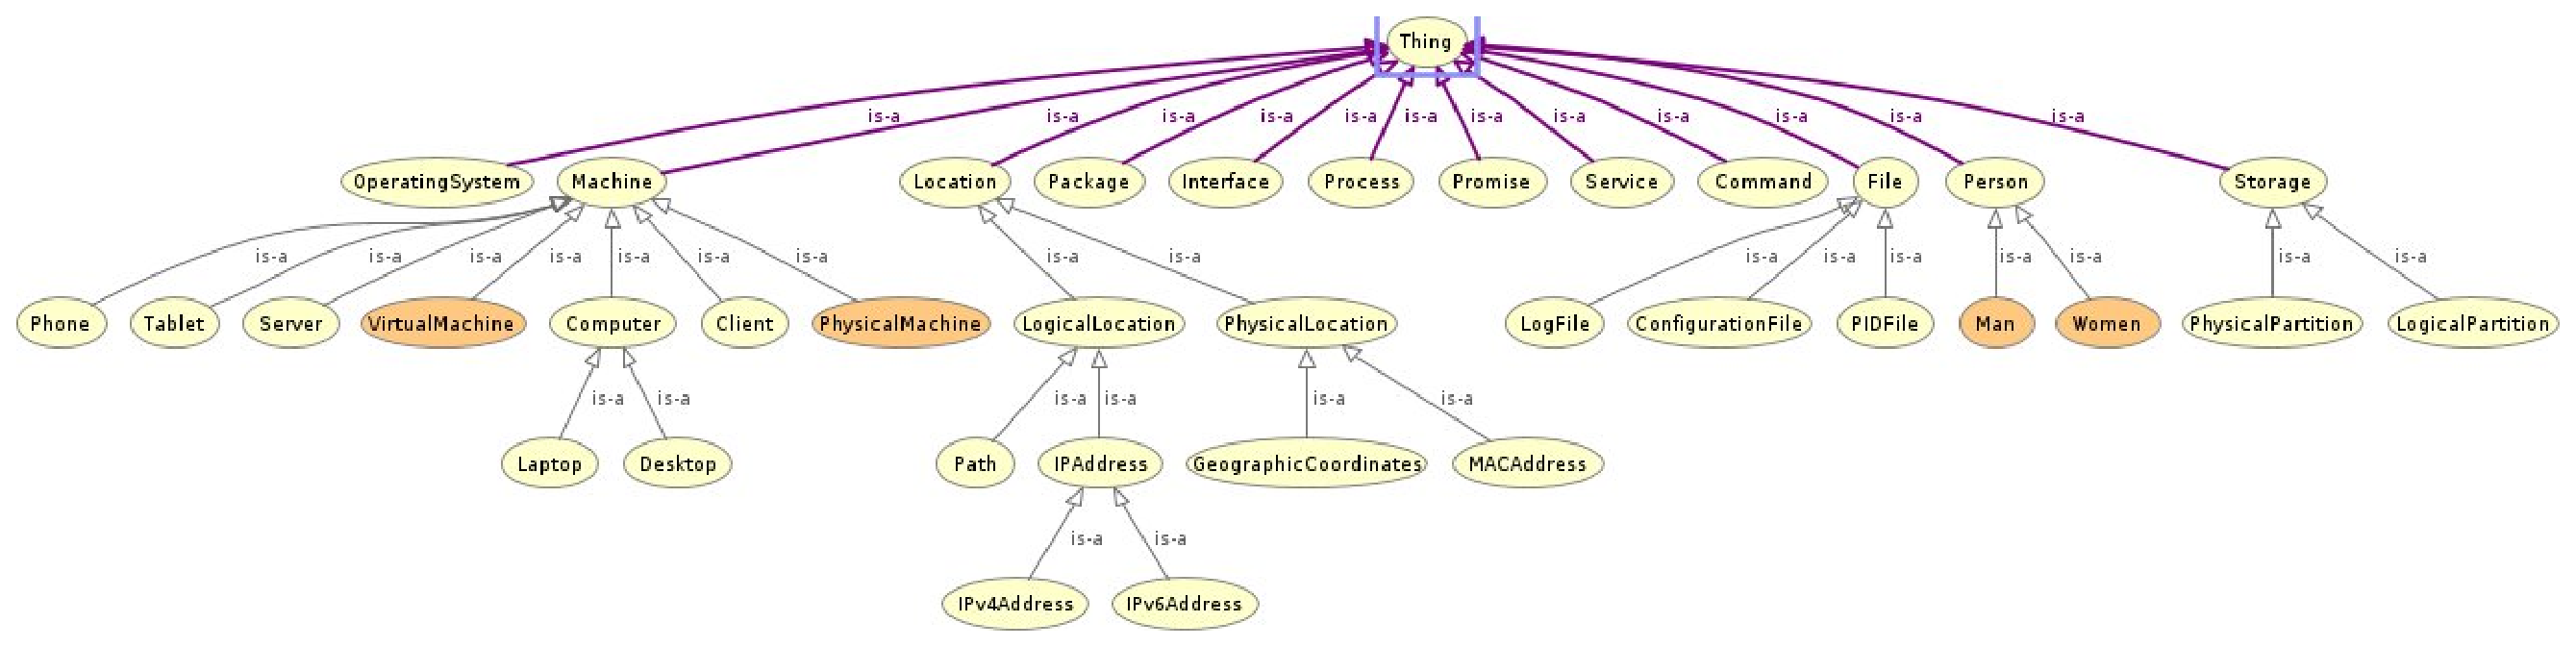
\includegraphics[width=\textwidth]{img/ontology_entities}
    \caption{Entités de l'ontologie}
    \label{fig:ontology_entities}
%\end{wrapfigure}
\end{figure}

\begin{itemize}
  \item \textbf{Machine} est n'importe quel périphérique en mesure d'accepter et
	  de traiter des informations pour fournir le résultat désiré basé sur
	  un programme ou une séquence d'instructions sur comment les données
	  doivent être traitées.
  \item \textbf{Computers} sont le type principal de machines dans cette étude.
	  C'est pourquoi les deux terminologies sont interchangeables dans
	  diverses sections de ces travaux. Les ordinateurs personnels (PCs),
	  les ordinateurs portables et les serveurs héritent tous de ce type.
  \item \textbf{Operating System} est un programme faisant le pont en les
	  composants logiciels et les composants matériels sous-jacents d'une
	  machine. Le système d'exploitation est une entité comportant plusieurs
	  sous-classes disjointes telles que Windows XP, OS X ou Linux.
  \item \textbf{Packages} sont les programmes applicatifs conçus pour servir un
	  but spécifique comme distribuer un service local, réseau ou web sur
      une ou plusieurs machines. Le paquet Apache est bon exemple d'entité
      conçue pour activer un service web.
  \item \textbf{Service} est une fonctionnalité spécifique d'un système
	  informatique comme un service web ou réseau offert par une machine. Un
	  processus qui est défini dans ce document comme un ensemble ou d'une
	  partie d'un ensemble de mesures permettant la fourniture de services
	  en exécutant des activités réelles en tâche de fond.
  \item \textbf{Command} est un utilitaire pouvant être utilisé par les
	  utilisateurs pour démarrer un processus spécifique, à la condition
	  qu'il n'existe pas de planification pour l'exécution de cette même
	  tâche. Un très bon exemple permettant d'illustrer cette relation
	  entre ces deux entités serait un web service, qui nécessite qu'un
	  processus tel que ''httpd'' soit démarré en arrière plan à l'aide de
	  la commande ''\begin{verbatim}httpd start\end{verbatim}''.
  \item \textbf{Storage} est une partition logique d'un média de stockage
	  physique qui sert principalement d'hôte pour les différents types de
	  fichiers. Un fichier est défini comme une collection d'informations
	  complète comme un programme, un ensemble de données utilisées par un
	  programme ou un document créé par un utilisateur.
  \item \textbf{Interface} est défini comme un périphérique permettant l'accès à
	  un réseau par une machine.
\end{itemize}

\subsubsection{Propriétés objets principales de l'ontologie (Relations)}

%\begin{wrapfigure}{r}{.7\textwidth}
\begin{figure}[h]
    \centering
    \begin{tabular}{p{.54\textwidth}p{.43\textwidth}}
        \noindent
        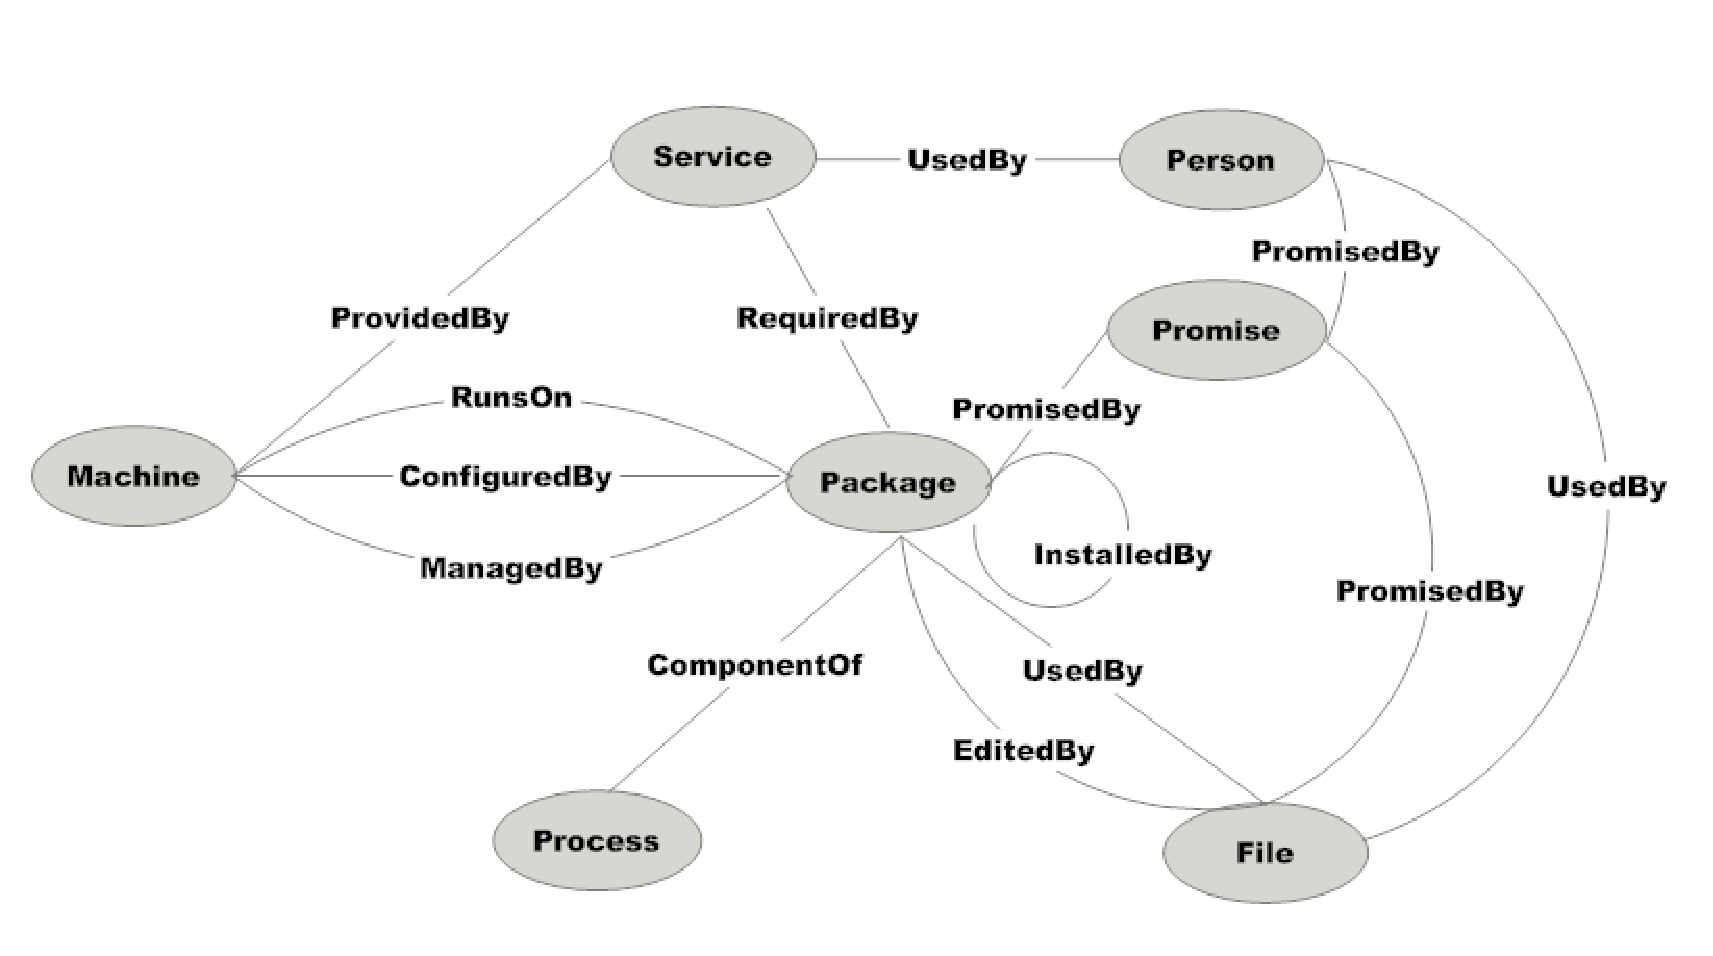
\includegraphics[width=.53\textwidth]{img/ontology_relations1}
        &
        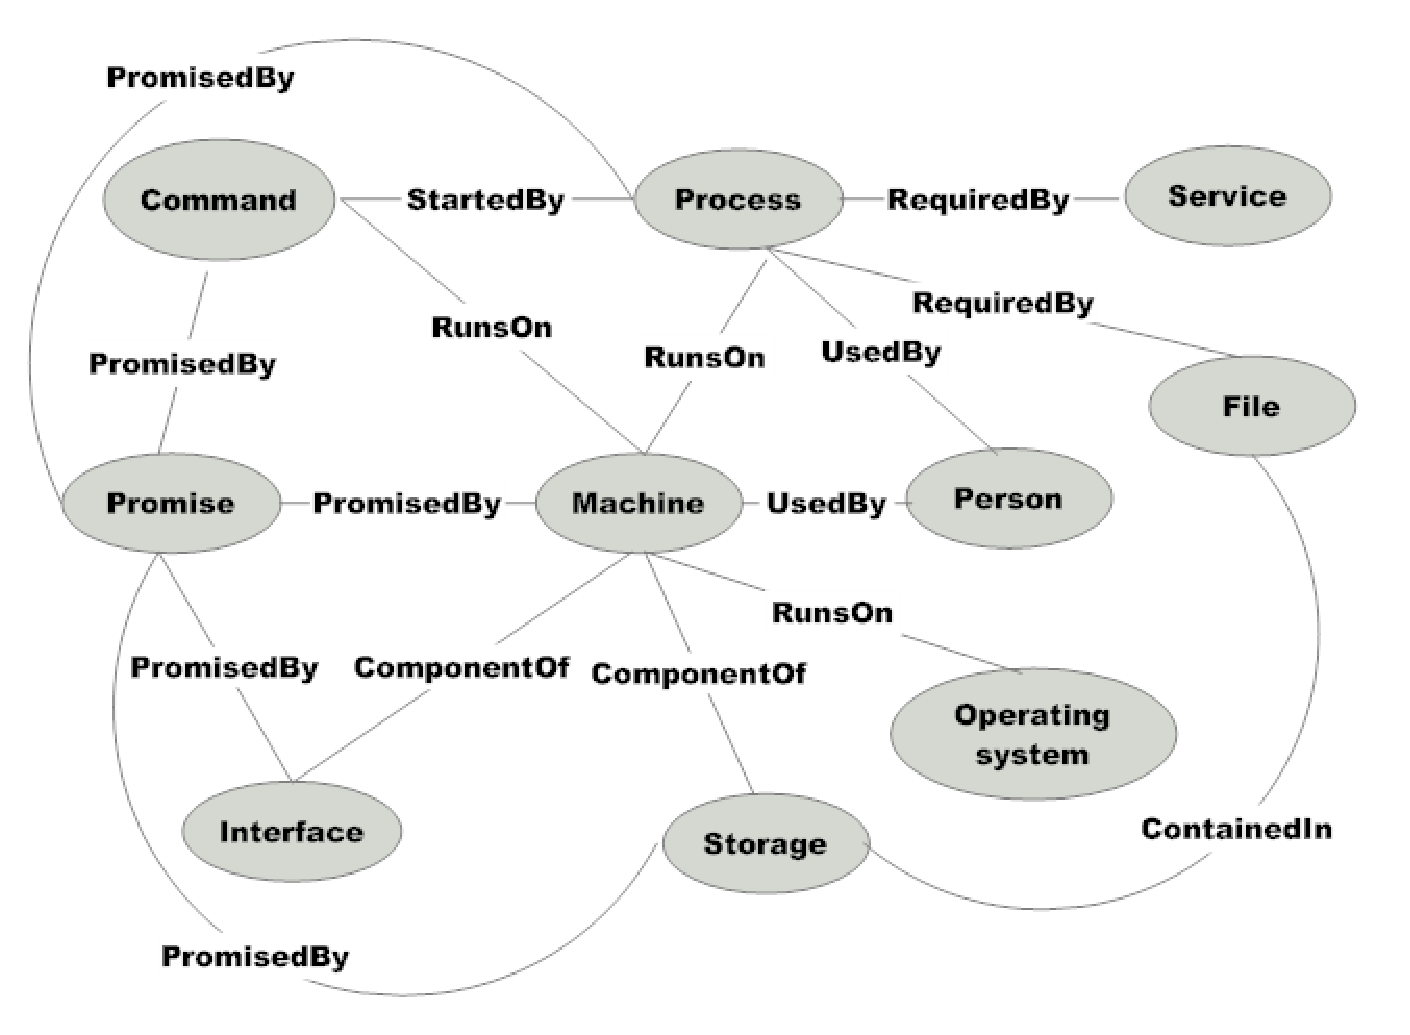
\includegraphics[width=.42\textwidth]{img/ontology_relations2}
    \end{tabular}
    \caption{Propriétés objets de l'ontologie}
    \label{fig:ontology_entities}
%\end{wrapfigure}
\end{figure}

\begin{itemize}
  \item \textbf{Caused By} :
          Un type d'association où une entité joue le rôle d'affecter l'autre en
	  changeant son état de l'état X à l'état Y.
  \item \textbf{Configured By} : 
	  Quand une entité X peux apporter les changements nécessaires à
	  l'entité Y pour lui permettre d'accomplir ses objectifs et ses
	  intentions. Le lien entre une machine et un progiciel de gestion de
	  configuration comme CfEngine 3 est un exemple typique de ce type de
	  relations.
  \item \textbf{Edited By} : 
	  Décrit qu'un fichier peut être modifié par un éditeur tel que
	  l'utilisateur du fichier à certaines fins.
  \item \textbf{Managed By} : 
	  Si X est responsable du bon fonctionnement de Y dans l'accomplissement
	  de son objectif, X est dit manager de Y. Le fait qu'une entité hérite
	  de ce rôle implique une supervision constante et des prises de mesures
	  lorsqu'intervient une déviation dans le comportement souhaité.
  \item \textbf{Monitoring By} : 
	  La supervision est principalement la responsabilité de garder un œil
	  sur quelque chose. Si une entité X supervise Y, elle surveille une
	  quelconque altération de comportement pour en informer le ou les
	  managers en charge de cette entité.
  \item \textbf{Component Of} : 
	  La relation entre une entité X, composante d'une entité plus globale Y
      qui joue le rôle d'encapsuleur pour ce composant X.
  \item \textbf{Owned By} : 
	  La propriété est un type de relation pouvant exister entre entité
	  devenue possession et son propriétaire. Le lien entre un fichier et son
	  propriétaire est un exemple de cet type d'association.
  \item \textbf{Promised By} : 
	  La relation en une promesse et l'entité qui la formule. 
  \item \textbf{Required By} : 
	  Si X dépend de Y dans l'accomplissement de ses intentions, la relation
	  entre ces deux entités est de type ''Required By''.
  \item \textbf{Runs On} : 
	  Si l'entité X exerce ses activités ou son exécution sur l'entité Y, la
	  relation est appelé ''Runs On''.
  \item \textbf{Written By} : 
	  La relation entre une écriture X et son auteur Y.
  \item \textbf{Used By} : 
	  Si une entité X fait l'usage d'une entité Y à n'importe quelle moment
	  de son exercice, la relation est de type ''Used By''.
  \item \textbf{Started By} : 
	  Quand une entité X est responsable du démarrage d'une entité Y ou
	  qu'elle commence à se comporter d'un certaine manière, l'association
	  est dite de type ''Started By''.
  \item \textbf{Provided By} : 
	  Quand une entité X a le potentiel et la bonne volonté de fournir
	  quelque chose à une autre entité Y, la relation entre ces deux entités
	  est appelée ''Provided By''.
  \item \textbf{Installed By} : 
	  Une entité X peut mettre en place un programme Y dans une machine de
	  manière à accomplir son but recherché. La relation existante entre X
	  et Y est alors de type ''Installed By''.
  \item \textbf{Contained In} :
	  Si une entité X est contenue dans Y, physiquement ou conceptuellement,
	  la relation est de type ''Contained In''.
\end{itemize}

\subsubsection{Propriétés de données principales de l'ontologie (Attributs)}

%\begin{wrapfigure}{r}{.7\textwidth}
\begin{figure}[h]
    \centering
    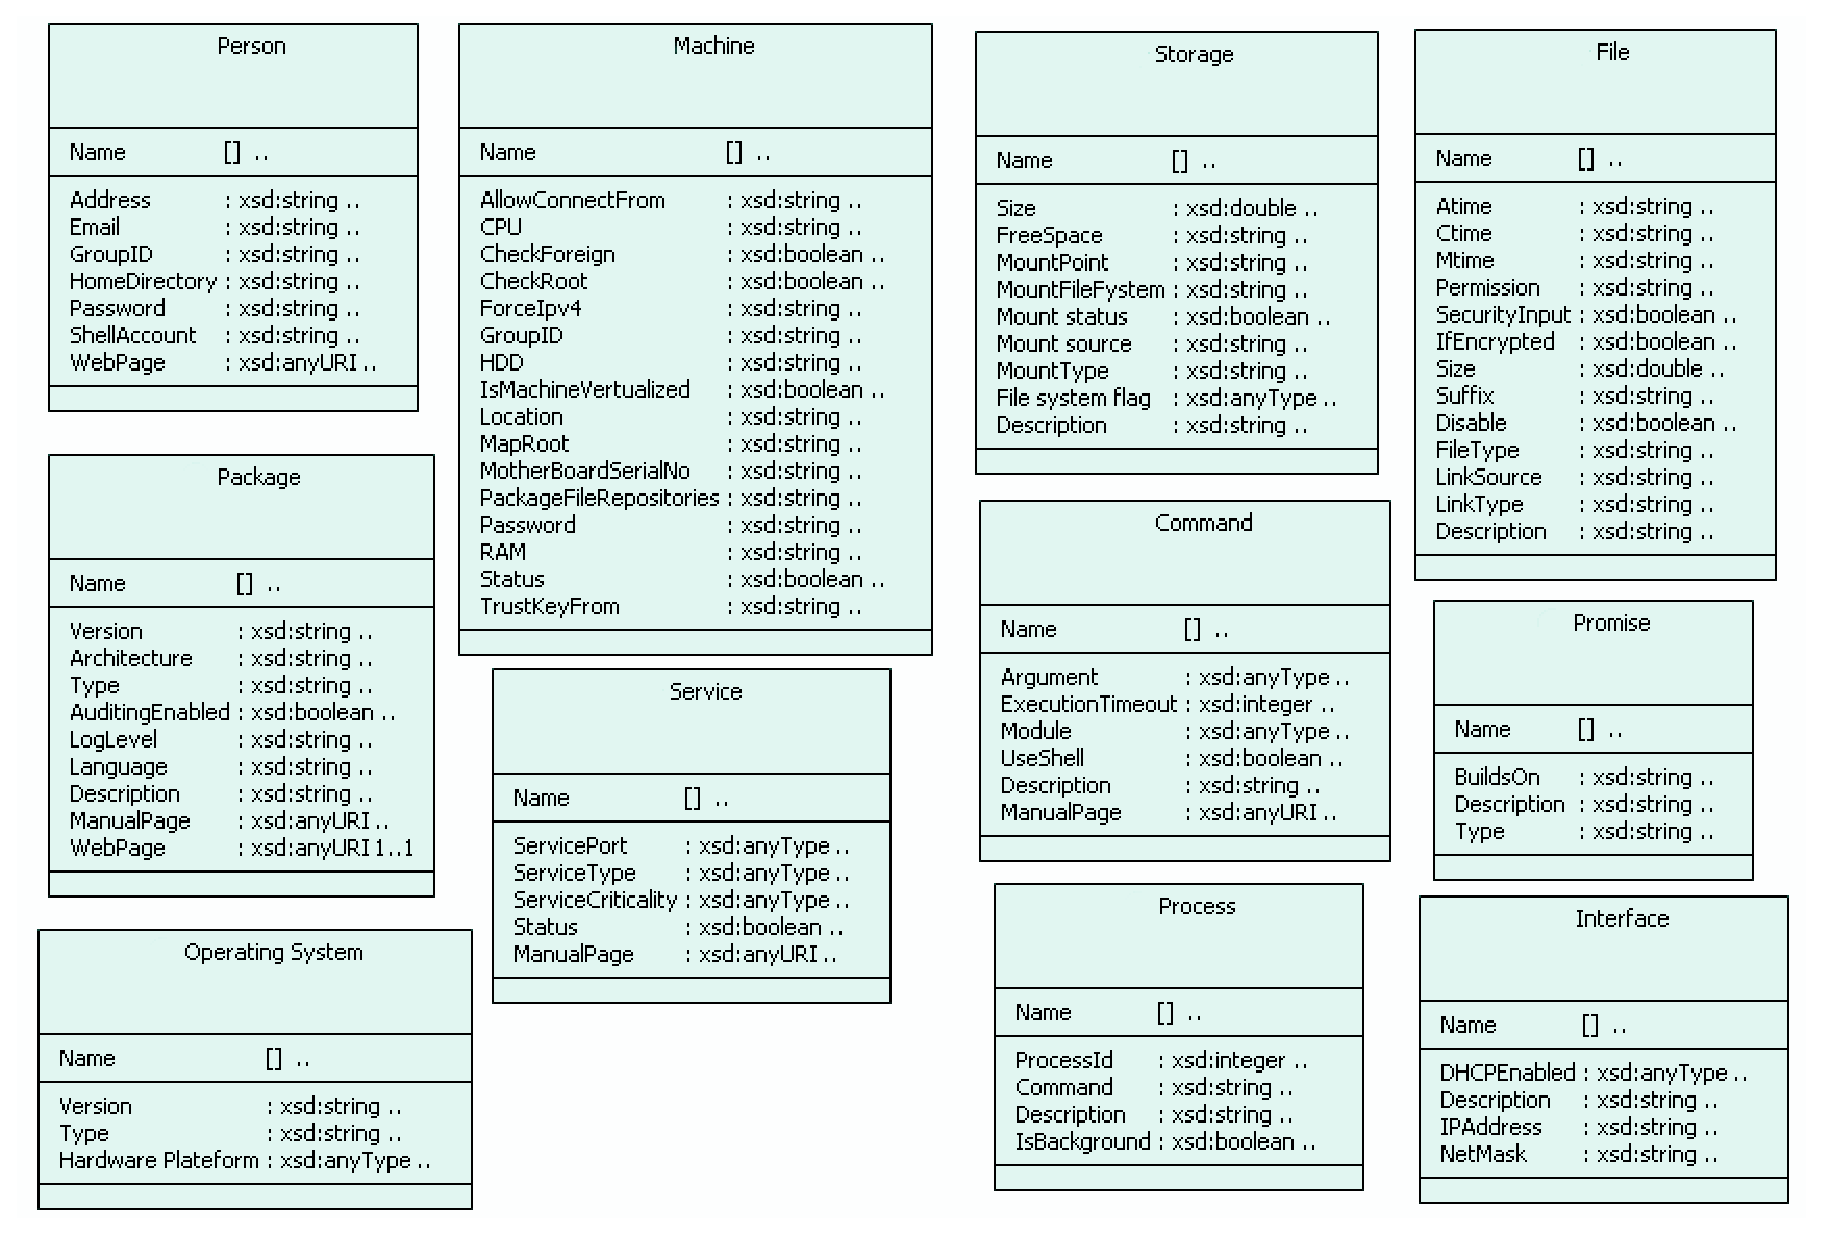
\includegraphics[width=.8\textwidth]{img/ontology_attributes}
    \caption{Propriétés de données de l'ontologie}
    \label{fig:ontology_entities}
%\end{wrapfigure}
\end{figure}

\begin{itemize}
  \item \textbf{AllowConnectFrom} : Liste d'adresses IP ou de nom d'hôtes
	  susceptibles d'avoir plus d'une connexion au port d'un serveur.
  \item \textbf{CheckForeign} : Indique s'il est nécessaire de vérifier les
	  autorisations sur le répertoire racine lors de la recherche de la
	  profondeur.
  \item \textbf{CheckRoot} : Liste de nom d'hôtes ou d'adresses IP auxquels
	  accorder un droit de lecture sur le serveur.
  \item \textbf{ForceIpv4} : Indique s'il y a un usage forcé de l'adresse IP
	  pour les connexions.
  \item \textbf{IsMachineVirtualized} : Indique si une machine est virtuelle ou
	  non.
  \item \textbf{PackageFileRepository} : Liste de répertoires locaux à la
	  machine pour la recherche de paquets.
  \item \textbf{TrustKeyFrom} : liste des hôtes pour lesquelles une machine
	  acceptera les clés publiques sur base de la confiance. Définition des
	  types d'occurrences qui sont liés avec le type d'entité stockage sont
	  répertoriés ci-dessous. Un stockage est une partition logique d'un
	  support de stockage physique.
  \item \textbf{FreeSpace} : Pourcentage minimum ou absolu d'espace disque
	  devant être disponible sur le support de stockage avec de lever un
	  avertissement.
  \item \textbf{MountType} : Type de protocole d'un système de fichier distant. 
  \item \textbf{FileSystemFlag} : Liste des options de menu à définir pour les
	  drapeaux de système de fichiers BSD. 
  \item \textbf{Atime} : Plage temporelle d'accès pour les fichiers
	  admissibles.
  \item \textbf{SecureInput} : Indique si les fichiers d'entrée sont accessibles
	  en écriture pour les utilisateurs non-autorisés.
  \item \textbf{MountType} : L'option de menu pour le type de liens à utiliser
	  lors de la copie comme le lien symbolique et le lien physique.
  \item \textbf{AuditingEnabled} : Indique si la fonctionnalité de journal
	  d'audit d'un paquet est activé ou non.
  \item \textbf{LogLevel} : Le niveau de rapport envoyé à syslog.
  \item \textbf{Architecture} : L'architecture relative à la section de paquets
	  comme ''x86-64'' ou ''i386''.
  \item \textbf{BuildsOn} : Liste de groupement de promesses sur lesquelles
	  s'appuie ou dépend une promesse d'une certaine manière (pour la
	  gestion des connaissances)
  \item \textbf{HomeDirectory} : Répertoire contenant les fichiers personnels
	  d'un utilisateur.
  \item \textbf{ShellAccount} : Compte personnel donnant accès à une invite de
	  commande Unix.
  \item \textbf{Module} : Indique s'il faut s'attendre à un protocole de module
	  CfEngine.
\end{itemize}

\subsubsection{Conception d'une ontologie de services}

Dans le but d'améliorer la compréhension globale, les aptitudes des différents
composants de l'infrastructure devront être formalisés à l'aide d'une ontologie
dédiée aux services. Celle-ci implémente trois concepts majeurs :

\begin{itemize}
    \item \emph{ServiceProfile} (partie ''Quoi'')
    \item \emph{ServiceModel} (partie ''Comment abstrait'')
    \item \emph{ServiceGrounding} (partie ''Comment concret'')
\end{itemize}

Tout comme pour la standardisation de la gestion intelligente de la
configuration, la classe \emph{ServiceModel} est très importante. Les services
sont modélisés comme des processus et la classe \emph{Process} est utilisée pour
indiquer les opérations à des niveaux de granularité différents. La classe
\emph{Process} comprend principalement deux types de processus : atomiques et
composites. Puisque l'information de gestion de configuration est définie comme
un ontologie OWL, l'information peut être utilisée comme les paramètres des
opérations de gestion de la configuration, qui sont définis sous la forme de
processus composites.  Chaque service de gestion de configuration correspond à
un processus composite, lui-même composé de plusieurs processus atomiques. Quand
le gestionnaire invoque un service de gestion de configuration prédéfini en
OWL-S, le service sera alors exécuté pour le dispositif réseau en place.

\section{Règles sémantiques et politiques de comportement}

Un autre domaine de recherche concernerait l'utilisation de règles pour exprimer
les comportements souhaités en termes d'éléments de haut niveau. Des langages
de définition de règles sont utilisés dans certains cas pour obtenir la
sensibilité au contexte. CRIME \cite{murphy_coordination_2007} par exemple, est
une implémentation prototypique du modèle Fact Space, qui est un langage de
coordination fournissant aux applications une vue de leur environnement. Les
règles CRIME décrivent le comportement des applications conformément à
l'information de contexte. CRIME traite également les déconnexions en invalidant
les faits et conclusions qui sont tirés des périphériques qui ne sont plus
disponibles dans l'environnement.

\subsection{Gestion basée sur des politiques (Policy-Based)}

La politique est identifiée comme une spécification de la configuration moyenne
du système sur des périodes persistantes. Un aspect important de cette
définition est qu'elle permet une certaine tolérance à l'erreur, nécessitée par
les évènements aléatoires se produisant susceptibles de corrompre la politique
en place dans la boucle de gestion du système. Il existe un élément probabiliste
ou stochastique pour le comportement du système et, par conséquent, la politique
ne peut être qu'une propriété moyenne en général.

\subsection{Choix d'un modèle de définition des politiques d'administration}

Le modèle permettant la définition des politiques d'administration serait un
modèle orienté sur les ontologies et basé sur la théorie de la promesse.
Celle-ci s'appuie sur un contrôle évolutif des objets intelligents,
contrairement aux modèles impératifs plus traditionnels pensés comme des
systèmes de gestion descendants. Dans ces derniers, le gestionnaire central
doit être informé des commandes de configuration des objets sous-jacents et de
l'état actuel de ces objets.

Au sein du contexte, le modèle fournit une série d'objets qui définissent
l'application. Les objets englobent les terminaux, les groupes de terminaux et
les politiques qui définissent leurs relations.

L'infrastructure conçoit un modèle d'objet pour le déploiement d'applications,
ces dernières constituant le point central. Historiquement, les applications
étaient limitées par les capacités du réseau et par des configurations visant à
prévenir leur utilisation abusive. Des concepts tels que l'adressage, le VLAN et
la sécurité sont depuis toujours intrinsèquement liés, ce qui limite
l'évolutivité et la mobilité des applications. Alors que les applications sont
redessinées pour la mobilité et l'évolutivité web, cette approche traditionnelle
empêche leur déploiement rapide et homogène.

\subsection{Théorie de la promesse}

La théorie de la promesse est une théorie nouvelle sur ce qu'il peut arriver
dans un réseau de composants entièrement autonomes.

Plutôt que d'adopter la croyance conventionnelle que ''seulement ce qui est
programmé peut arriver'', elle prend le point de vue opposé : ''seulement ce
qui est promis peut être prédit''. Elle aborde donc la gestion du point de vue
de l'incertitude avec réalisme plutôt que celui de la foi en la conformité. Dans
la théorie de la promesse, on suppose un point de vue orienté service des
interactions entre les différents dispositifs informatiques. Chaque nœud propose
de jouer un rôle dans un réseau de collaboration en promettant de restreindre
son comportement de différentes manières. Une utilisation typique de la théorie
de la promesse est d'examiner le comportement en régime permanent d'un certain
nombre d'agents (composants) autonomes. La théorie de la promesse ne détermine
pas nécessairement pleinement le comportement de ses composants, elle représente
seulement les contraintes au sein d'un ensemble de comportements définis. Elle
n'est pas limitée aux promesses linéaires.

La théorie de la promesse adhère à un point de vue orienté service des
politiques des gestion et utilise un langage graphique pour composer et analyser
les propriétés systèmes.

Une caractéristique essentielle des promesses est qu'elles séparent clairement
ce qui contraint et à qui la contrainte s'applique. C'est un autre domaine qui
soulève bien souvent des confusions dans la théorie des politiques. Néanmoins,
le modèle ontologique permet un fois de plus de bien distinguer ces deux
aspects grâce à son haut degré de formalisme.

\subsubsection{CfEngine3: une implémentation de référence de la théorie de la
promesse}

CfEngine3 implémente deux approches :

\begin{itemize}
    \item \textbf{Centralisée}: 
        le système va pousser avec force les règles et règlements établis de
        manière centralisée avec ou sans la volonté de l'utilisateur final hôte.
    \item \textbf{Basé sur des politiques} :
        cette approche fonctionne de la même manière que le protocole SNMP
        (Simple Network Management Protocol), à l'exception qu'elle donne une
        autonomie totale aux agent, de manière à ce qu'ils aient plein droit de
        tirer et implémenter un ensemble centralisé de politiques de
        configuration.
\end{itemize}

En théorie, chacun des agents autonomes va faire formuler une promesse sur le
comportement qu'on attend de lui, basé sur un choix qui lui est propre. C'est ce
que rend la théorie de la promesse optimale pour un framework de gestion basé
sur des politiques.

La théorie de la promesse décrit des services régis par des politiques, dans un
framework d'agents complètement autonomes, qui s'entraident les uns les autres
seulement par une coopération volontaire. Dans CfEngine3, chaque élément de
configuration va faire une promesse concernant ses caractéristiques propres et
sa relation avec d'autres éléments de configuration.

Nous souhaitons être en mesure de promettre que le système est cohérent, de le
vérifier et d'effectuer des changements seulement si des promesses ne sont pas
tenues. Cela nécessite, en plus de l'implémentation initiale de ces promesses,
la vérification continue de l'état de chacun des éléments de configuration
vis-à-vis de leur promesses respectives pour assurer un système cohérent et en
conformité avec les politiques en vigueur.

% TODO : expliquer ITIL
%Pour comprendre ITIL (Information Technology Infrastructure Library), il
%faut l'imaginer comme un service fourni par CfEngine.

\subsection{Gestion de configuration basée sur la théorie de la promesse}

\subsubsection{Données paramètres}

Un système de gestion de configuration basé sur la théorie de la promesse
accepte comme paramètres d'entrée un ensemble de politiques de configuration de
haut niveau. Ces politiques de haut niveau seront divisées en spécifications de
configuration de bas niveau, que nous appellerons ``promesses`` dans la
modélisation par la théorie de la promesse. Notre ontologie permettra la
formalisation de ces promesses.

En complément des politiques de configuration, les informations suivantes
pourront être transmises au système de gestion de configuration :

\begin{itemize}
    \item Le nombre et le type de machines nécessaires
    \item Le système d'exploitation de chacune des machines
    \item Les paquets ayant besoin d'être installés sur chaque machine
    \item Les services que chacun des hôtes doit fournir
    \item Les préoccupations liées au stockage comme le type de système de
        fichiers
    \item Les questions de sécurité, incluant notamment les aspects de gestion
        des utilisateurs
\end{itemize}

\subsubsection{Traitements}

Les politiques de configuration de haut niveau subiront deux traitements
majeurs. Le premier concerne la spécification de la configuration de bas
niveau. Ce traitement dépend de l'information liée à l'architecture telle que le
détail du périphérique ou le type de topologie attendu par un système.
Le deuxième consiste à respecter les promesses formulées par chacun des éléments
de configuration. Ce traitement s'assure que chaque élément de configuration se
comporte conformément à ses promesses. Dans la gestion des changements,
CfEngine3 prendra des mesures correctives en plus de jouer le rôle d'informer
les parties concernées en cas de non tenue d'une promesse.

\subsubsection{Résultats attendus}

Le résultat de ces traitements est un système conforme aux règles politiques en
vigueur où chaque élément de configuration possèdent les clés et valeurs
attendues.  Autrement dit, un ensemble d'ordinateurs avec les valeurs de
configuration appropriées (les valeurs d'attribut promises).  Les éléments de
configuration principaux sont les fichiers, les paquets, les disques, les
processus, le services et les interfaces. 

En plus de leurs propres valeurs d'attributs et manière d'agir, un ensemble de
promesses sur le bon type de relations entre ces éléments de configuration est
nécessaire pour valider le résultat de ces traitements.

\section{Consistance de l'information et tolérance à l'échec}

\subsection{Choix d'un algorithme de consensus}
\label{sec:consensus}

Le consensus est un problème fondamental dans les systèmes distribués tolérants
aux pannes. Un consensus implique de multiples serveurs acceptants des valeurs.
Une fois qu'ils atteignent une décision sur une valeur, cette décision est
définitive. Les algorithmes de consensus typiques sont amenés à faire des
progrès lorsque la majorité de leurs serveurs sont disponibles, par exemple, un
cluster de 5 serveurs peut continuer à fonctionner même si deux serveurs ne sont
plus disponibles. Si plusieurs serveurs échouent, ils cessent de faire des
progrès, mais ils ne retournerons jamais de valeurs erronées.

\subsubsection{Choix du consensus de Raft}

Raft est un algorithme de consensus qui est conçu pour être facile à comprendre.
Il est équivalent à Paxos dans la tolérance aux pannes et en termes de
performances. La différence est qu'il est décomposé en sous-problèmes
relativement disjoints, et traite de manière rigoureuse toutes les pièces
majeures nécessaires pour obtenir un système cohérent.

Il existe des écarts significatifs entre la description de l'algorithme de Paxos
et les besoins d'un système dans le monde réel. Le système au final serait basé
sur un protocole dénué de preuves.

\begin{table*}
    \begin{tabular}{p{.48\textwidth}p{.48\textwidth}}
        \noindent
        \textbf{\textit{Inconvénients de Paxos}}
    
        \begin{itemize}
            \item Extrêmement difficile à comprendre. L'opacité de Paxos dérive
                de son choix d'avoir un sous-ensemble de décrets uniques comme
                son fondement.
            \item Ne fourni pas une bonne base pour la construction
                d'applications pratiques. Par exemple, il y peu d'avantages à
                choisir de manière indépendante une collection d'entrées dans le
                registre, pour les fusionner par la suite dans un journal
                séquentiel ; cela ajoute seulement de la complexité. Il est plus
                simple et plus efficace de concevoir un système autour d'un
                journal, où les nouvelles entrées sont ajoutées séquentiellement
                dans un ordre contraint.
            \item Utilise une approche symétrique pair-à-pair à sa base. Cela a
                un sens dans un monde simplifié où seule une décision sera
                prise, mais peu de systèmes concrets utilisent cette approche.
                Si une série de décisions doivent être prises, il est plus
                simple et plus rapide d'élire d'abord un leader, puis de le
                laisser coordonner les décisions.
        \end{itemize} 
        
        &
    
        \textbf{\textit{Avantages de Raft}}
    
        \begin{itemize}
            \item Raft utilise une forme plus solide de leadership que les
                autres algorithmes de consensus. Par exemple, les entrées du
                registre ne seront communiquées que par le leader vers les autres
                serveurs. Cela simplifie largement la gestion de la réplication
                des journaux et rend Raft beaucoup plus facile à comprendre.
            \item Raft utilise des minuteries aléatoires pour élire les leaders.
                Cela ajoute un peu de mécanismes au système de pulsation déjà
                nécessaire dans n'importe quel algorithme de consensus, tandis
                que la résolution des confits se fait simplement et rapidement.
            \item Le mécanisme de Raft pour changer l'ensemble des serveurs de
                la grappe utilise une nouvelle approche de consensus conjointe
                où les majorités des deux différentes configurations se
                superposent pendant les transitions. Cela permet au groupe de
                continuer à fonctionner normalement pendant les changements de
                configuration.
        \end{itemize}
    
    \end{tabular}
    \caption{Comparaison des algorithmes de consensus de Raft et de Paxos}
    \label{table:consensus_comparison}
\end{table*}

\subsubsection{Caractéristiques des algorithmes de consensus}

Les algorithmes de consensus pour les systèmes concrets ont généralement les
caractéristiques suivantes :

\begin{itemize}
    \item Ils assurent la sécurité (ne retournent jamais de résultat erroné)
        sous toutes conditions non byzantines, y compris les retards dans le
        réseau, les pertes de partitions et de paquets, la duplication et
        la réorganisation.
    \item Ils sont entièrement fonctionnels (disponibles) dans la mesure où au
        moins la majorité des serveurs sont opérationnels et peuvent communiquer
        les uns avec les autres et avec les clients. Ainsi, un groupe type de
        cinq serveurs peut tolérer la défaillance de deux ses membres. Les
        serveurs sont supposés tomber en panne en s'arrêtant ; ils pourront plus
        tard retrouver un état stable et rejoindre le cluster.
    \item Il ne dépendent pas de la contrainte temporelle pour assurer la
        cohérence des journaux : des horloges défectueuses et des retards
        abusifs dans la délivrance des messages peuvent causer des problèmes de
        disponibilité. 
    \item Dans le cas le plus courant, une commande peut s'achever aussitôt que
        la majorité de la grappe a répondu à un seul tour d'appels à procédures
        distantes ; une minorité de serveurs lents ne doivent pas impacter les
        performances globales du système.
\end{itemize}

\subsubsection{Architecture de machines à états répliquées}

%\begin{wrapfigure}[8]{r}[0pt]{.4\textwidth}
\begin{figure}[h]
    \centerline{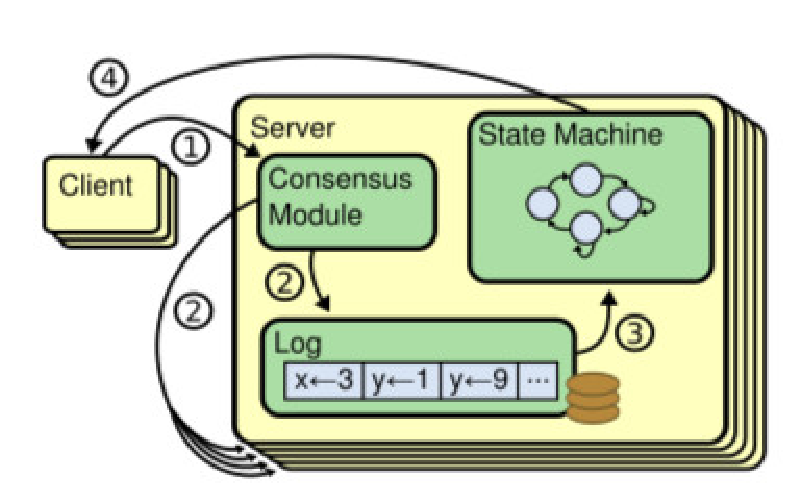
\includegraphics[width=.37\textwidth]{img/replicated_state_machine}}
    \caption{Procédé de réplication des machines à états}
    \label{replicated_state_machine}
%\end{wrapfigure}
\end{figure}

L'algorithme de consensus gère un registre répliqué regroupant les commandes de
la machine à états de chacun des clients dans le réseau. Les machines à états
traitent des séquences identiques de commandes à partir de journaux partagés, de
sorte qu'ils produisent les mêmes résultats.

Les systèmes à grande échelle n'ayant qu'un seul cluster leader utilisent une
machine à état distincte pour gérer les élections et pour stocker les
informations de configuration qui doivent survivre aux crashs du leader
(exemples: Chubby, ZooKeeper).

%\begin{verse}
%    \underline{
        Garder le registre répliqué consistant est le travail de l'algorithme de
        consensus.
%    }
%\end{verse}

\section{Conclusion}

Les différents concepts détaillés dans ce chapitre nous permettent de répondre
aux problématiques énoncées. L'ontologie apporte le haut degré de formalisation
nécessaire pour modéliser les informations de contexte et les promesses
permettant la définition des politiques de configuration du système.  La théorie
de la promesse propose une approche sémantique de la configuration, promettant
aux utilisateurs un travail de configuration à moindres efforts.  L'algorithme
de consensus garantit la tolérance à l'échec et une organisation rigoureuse des
communications inter-agents par l'attribution de rôles dans le cluster. Le
modèle de réplication des journaux qu'il implémente permet d'assurer la
permanente consistance de l'ontologie avec une simplicité remarquable.

% ex: set spelllang=fr spell: %
%%% Local Variables: ***
%%% mode: latex ***
%%% TeX-master: "thesis.tex" ***
%%% End: ***
